\section{Future Work}

While our implementation represents a significant step forward, the project offers ample opportunity for future expansion. %, including optimization of the physics engine, exploration of new biomes, items and game modes, and introduction of multiplayer capabilities. 
%Although our implementation could have been more performant had we used flecs, we opted for a design that allows continuous forwards-facing evolution of the game and is easy to work with for us and possibly other developers.
%
Therefore, we want to mention some concrete examples and ideas that can be used as starting point for the further development.
New items can be added such as a pickaxe or a gun that can shatter rocks.
Competitiveness between players could be introduced with a leaderboard.
Different biomes with different visuals and terrain generation can be implemented.  
Another option is to offer difficulty settings to the user and implementing a coin shop for buying upgrades.
Moreover, we propose a multiplayer mode where there are two hikers competing for who gets furthest and interacting with each other.
Alternatively, one player could play as the monster and throw snowballs at the hiker.
%The implementation of this mode requires the consideration of how players interact and how to resolve several aspects, e.g. the potential for player interaction and the resolution of scenarios such as the death of one player.

Our physics engine also offers various extension points.
One known issue with the way our physics are currently implemented is that we assume there are only vertex-face collisions as shown in fig. \ref{fig:SAT}.
However, edge-edge collisions can occur resulting in a jittering effect when rocks are stationary on the ground (see fig. \ref{fig:jitter}) due to falsely introduced torque.
Although this does not constitute a problem for our bouncy physics right now, we are aware that this will need to be solved if the game is to be extended with less bouncy entities.
Catto \cite{cattoManifolds} and Wheeler \cite{wheelerCD} show how to handle this effect using \emph{collision manifolds}.
The idea is to consider up to two colliding points between polygons and applying a combined impulse at an average contact point of the two colliding points weighed by their collision depth.

Another way of extending the physics engine would be to add friction or air resistance.
Friction can be modelled as two constants for static and dynamic friction.
A friction impulse is then applied during collisions in reverse tangential direction to $\vec{v}_{rel}$.
For the magnitude, simply replace the normal $\vec{n}$ with the tangent $\vec{t}$ in equation \ref{eq:scary}.
We implemented friction but decided against using it as it would currently negatively impact gameplay, which requires bouncy rocks.

Lastly, there are opportunities to further enhance the performance of the physics engine, e.g. by implementing parallel batch processing and spatial data structures.

% \subsection{Future Work}

% The physics engine we developed is suitable for our purpose and can be easily extended.



% To summarize, our physics engine provides a modular and highly extensible framework that can be built upon in many ways.
% It is suitable for small games and can be easily adapted to any small game that needs to simulate rigid convex polygons.

\begin{figure}[h!]
  \centering
  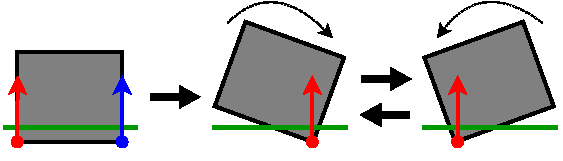
\includegraphics[width = .7\linewidth]{figures/physics/jitter.pdf}
  \caption{An edge-edge collision should consider more than one contact point in order to accurately resolve the collision. Here, the blue collision point is ignored and jitter is introduced.}
  \label{fig:jitter}
\end{figure}